% !TeX root = ../Book1.tex
\begin{figure}[htbp]
	\centering
	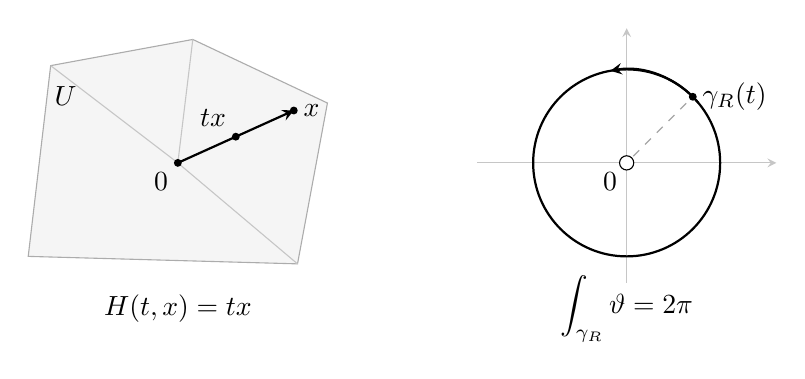
\begin{tikzpicture}[>=stealth,scale=0.95]
		\begin{scope}
			\filldraw[fill=gray!8,draw=gray!65] (-2,-1.25)--(-1.7,1.3)--(0.2,1.65)--(2,0.8)--(1.6,-1.35)--cycle;
			\node at (-1.5,0.9) {\(U\)};
			\draw[gray!45] (0,0)--(-1.7,1.3);
			\draw[gray!45] (0,0)--(0.2,1.65);
			\draw[gray!45] (0,0)--(1.6,-1.35);
			\draw[thick,->] (0,0)--(1.55,0.7);
			\fill (0,0) circle (1.5pt) node[below left] {\(0\)};
			\fill (0.775,0.35) circle (1.5pt) node[above left] {\(tx\)};
			\fill (1.55,0.7) circle (1.5pt) node[right] {\(x\)};
			\node at (0,-1.95) {\(H(t,x)=tx\)};
		\end{scope}
		\begin{scope}[xshift=6cm]
			\draw[gray!45,->] (-2,0)--(2,0);
			\draw[gray!45,->] (0,-1.6)--(0,1.8);
			\draw[thick] (0,0) circle (1.25);
			\draw[thick,->] (40:1.25) arc (40:100:1.25);
			\draw[dashed,gray!70] (0.09,0.09)--(45:1.25);
			\filldraw[fill=white,draw=black] (0,0) circle (2.7pt);
			\node[below left] at (0,0) {\(0\)};
			\fill (45:1.25) circle (1.5pt);
			\node[right] at (45:1.25) {\(\gamma_R(t)\)};
			\node at (0,-1.95) {\(\displaystyle\int_{\gamma_R}\vartheta=2\pi\)};
		\end{scope}
	\end{tikzpicture}
	\caption{左图中，从 \(0\) 到 \(x\) 的径向路径始终留在星形区域内，因此可以沿这一族路径构造原形式。右图的原点被删去，径向收缩不能到达原点；角形式沿圆周的非零周期进一步证明它没有整体原函数。}
	\label{g1:fig:radial-and-period}
\end{figure}
